\documentclass[aspectratio=169,notes]{beamer}
\usepackage[utf8]{inputenc}
\usepackage{booktabs}
\usepackage{multimedia}
\usepackage{graphicx}
\usepackage{caption}
\usepackage[backend=biber,style=verbose,autocite=footnote]{biblatex}
\addbibresource{references.bib}

\usetheme[progressbar=frametitle,block=fill]{metropolis}
\metroset{background=dark}
\setbeamerfont{note page}{size=\tiny}
\setbeamertemplate{navigation symbols}{}

\title{Sentiment And Network Analysis of Political Discussion on Reddit.com}
\subtitle{During the U.S.A. Presidential Election of 2012}
\author{João António Fernandes da Costa\inst{1}, \href{malito:bio12046@fe.up.pt}{bio12046@fe.up.pt}}
\institute[FEUP]
{
  \inst{}%
  Data Mining II\\
  Masters in Modeling, Data Analysis and Decision Support Systems\\
  School of Economics and Management\\
  University of Porto\\
  \inst{1}%
  Masters in Bioengineering\\
  Faculty of Engineering\\
  University of Porto\\
}
 
\date{\today}
 
\begin{document}
\frame{\titlepage}

\section{Introduction}

\begin{frame}{Introduction}
\begin{columns}
\begin{column}{.5\textwidth}
 Traditional social media can define discussion topics and narrative they want to push.
 
 \hspace{0pt}
 
 The growth of the Internet and \alert{Social News Web Sites} challenge the traditional media by being user-moderated.
\end{column}\pause

\begin{column}{.5\textwidth}
Social News Web Sites are platforms where:
\begin{itemize}
 \item Users generate or submit links to content;
 \item Submissions are voted and ranked accordingly;
 \item Users comment on submitted content;
 \item Comments are voted and ranked accordingly.
\end{itemize}
Examples of these sites are Reddit, Digg, (Facebook), ...
\end{column}
\end{columns}

\end{frame}

\note[itemize]{
\item O grande crescimento dos meios de comunicação digitais permitiu o aparecimento de websites de 'social news', que representam um distanciamento com os meis de comunicação tradicionais: ao passo que previamente uma organização noticiosa poderia definir os tópicos de discussão e coordenar a narrativa, hoje em dia, estes sites de comunidades digitais permitem a depuração, avaliação e apresentação de conteúdos relevantes para as massas, usando para isso o poder das massas. 
\item Usualmente este tipo de site permite aos utilizadores gerar ou submeter links para conteúdo que achem interessante, sendo essas submissões votadas pelo resto dos utilizadores. Os utilizadores também podem comentar essas submissões e os próprios comentários podem ser também votados e ordenados de acordo.
\item Existem vários exemplos deste tipo de site, como por exemplo Reddit, Digg, HackerNews e até um certo ponto o Facebook.
}


\begin{frame}{Reddit.com}
\begin{columns}
\begin{column}{0.5\textwidth}
Reddit.com is an American social news website created in 2005, the 6\textsuperscript{th} most popular website in the world\footnotemark.

Users can post, comment and upvote/downvote content.

The community is divided into specialized forums: \textit{subreddits}.
\end{column}

\begin{column}{0.5\textwidth}
\begin{figure}[htp]
 \centering
 
\includegraphics[width=\linewidth]{reddit_screenshot.png}
 \caption{Reddit Homepage}
 \label{fig:reddit}
\end{figure}
\end{column}
\end{columns}
\footcitetext{ref:alexa}

\end{frame}
\note[itemize]{
\item O site Reddit.com é um exemplo de um desses sites de 'social news'. Criado em 2005 nos EUA, é atualmente o 6º website mais popular do mundo.
\item Nele, os seus utilizadores podem submeter conteúdo ou links e comentar outras submissões. Para além disso, os utilizadores podem anonimamente votar para cima ou para baixo (upvote/downvote) submissões e comentários.
\item Outra caraterística fundamental para o entendimento do Reddit é a sua divisão em subreddits. Subreddits são fóruns mais específicos que incidem num tópico particular, criados e moderados por utilizadores. Utilizadores podem subscrever a um subreddit específico para visualizar o seu conteúdo na sua homepage. Os maiores subreddits fazem parte da lista de autosubscrições, que todos os utilizadores partilham e visualizam.
}

\begin{frame}{U.S. Presidential Election 2012}
 \begin{columns}
 \begin{column}{0.5\textwidth}
\begin{figure}[p]
 \centering
 \colorbox{white}{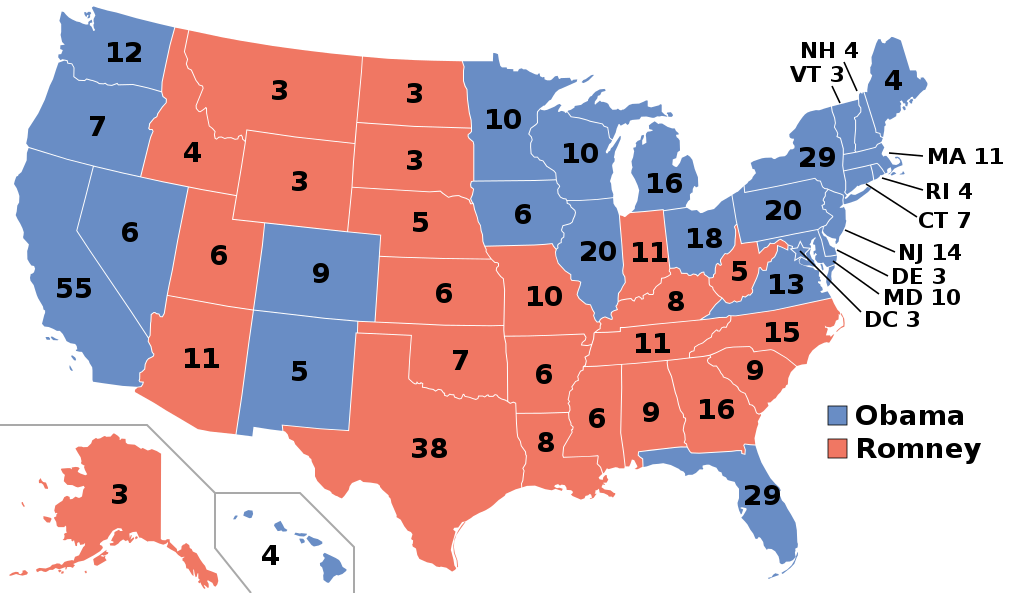
\includegraphics[width=\linewidth]{ElectoralCollege2012.png}}
 \captionsetup{justification=centering}
 \caption{Electoral College map for the 2012 United States presidential election\footnotemark}
\end{figure}

\end{column}

\begin{column}{0.5\textwidth}
\alert{Barack Obama} and Joe Biden (Democratic Party)

vs. Mitt Romney and Paul Ryan (Republican)

\begin{block}{Electoral Votes}
 332 Democratic vs. 206 Republican
\end{block}

\begin{block}{Popular Vote}
 51.1\% Democratic vs. 47.2\% Republican
\end{block}

\begin{block}{Turnout - 54.9\%}
\end{block}

\end{column}
\end{columns}
\footcitetext{nytimes_election}
\end{frame}

\begin{frame}{Vote Intention Evolution}
 \begin{figure}[p]
 \centering
 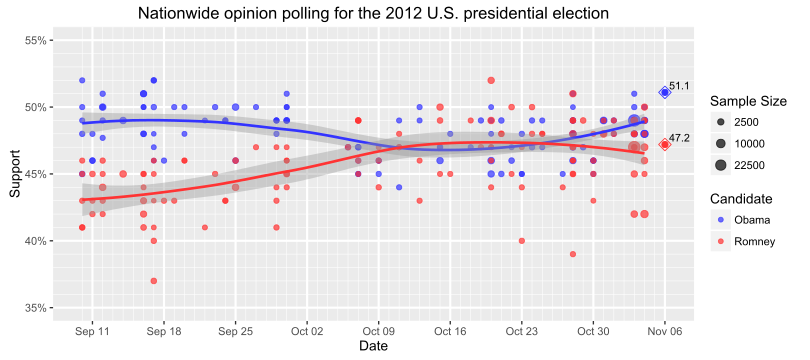
\includegraphics[width=\linewidth]{time_intention.png}
 \captionsetup{justification=centering}
 \caption{Summary of the opinion polls taken since convention nominations for the U.S. presidential election}
\end{figure}
\end{frame}

\begin{frame}{Python}
 \alert{Python 3.6} was used to process downloaded data, process comments, perform sentiment analysis and plot resulting graphics.
 
 Relevant packages used:
 \begin{description}
  \item[SKLearn] for text-mining feature extraction
  \item[NLTK] Natural Language Toolkit, for stemming and sentiment analysis (VADER)
  \item[NetworkX] for Graph analysis and export
 \end{description}
\end{frame}

\begin{frame}{Challenges}
 Can we distinguish different political \alert{subreddits} based on their \alert{comment's text} content and general \alert{sentiment} to the candidates?\pause
 
 Can we detect important \alert{events} that changed the public's opinion based on the general \alert{sentiment} of comments?
\end{frame}

\section{Dataset Description}

\begin{frame}{Comments and Submissions}
 Posts and comments from October 2012 are downloaded\footnotemark
 
 Posts and comments are parsed by subreddit:
 
 \begin{block}{Considered Subreddits, by order of activity}
  r/politics, 
  r/PoliticalDiscussion, 
  r/Conservative, 
  r/Libertarian, 
  r/Republican, 
  r/PoliticalHumor, 
  r/obama, 
  r/Romney, 
  r/democrats
 \end{block}
\footcitetext{reddit_download}
\end{frame}

\begin{frame}{Dataset Statistics}
 \begin{table}[]
\centering
\caption{Statistics of collected Reddit Dataset}
\begin{tabular}{@{}lll@{}}
\toprule
Subreddit                    & \# of Posts & \# of Comments \\ \midrule
\textbf{politics}            & 3665        & 128275         \\
PoliticalDiscussion          & 1127        & 39445          \\
\textbf{Conservative}        & 767         & 26845          \\
Libertarian                  & 712         & 24920          \\
Republican                   & 254         & 8890           \\
PoliticalHumor               & 83          & 2905           \\
obama                        & 52          & 1820           \\
Romney                       & 29          & 1820           \\
democrats                    & 18          & 630            \\ \bottomrule
\end{tabular}
\end{table}
\end{frame}

\section{Preprocessing of Data}

\begin{frame}{Tokenization and Stemming}
\begin{columns}
 
\begin{column}{.5\textwidth}
 \begin{block}{Comment Preprocessing}
 \begin{itemize}
  \item Turned to lowercase
  \item Punctuation removed
  \item Only alphabetic strings considered
  \item Stopwords removed
  \item Words with 2 or less letters removed
 \end{itemize}
 \end{block}
\end{column}

\begin{column}{.5\textwidth}
 \begin{block}{Comment Stemming}
  Snowball Stemmer
 \end{block}
\end{column}
\end{columns}
\textit{Yet that moron capitalizes on every subsidy she publicly denounces.}

\textit{['yet', 'moron', 'capitalizes', 'every', 'subsidy', 'publicly', 'denounces']}

\textit{['yet', 'moron', 'capit', 'everi', 'subsidi', 'public', 'denounc']}
\end{frame}

\begin{frame}{Dictionary-Based Categorization of Comments}
\begin{exampleblock}{Democrat Dictionary}
 obama, biden, liber, barack, joe, democrat, dem, libtard, obamacar, left, lefti, leftist
\end{exampleblock}
\begin{exampleblock}{Republican Dictionary}
 republican, republ, conserv, conservat, gop, mitt, romney, paul, ryan, right
\end{exampleblock}

Each processed comment is analysed against both dictionaries: if it contains a word of a certain dictionary, it is labelled as such.

Afterwards, only comments belonging to a \alert{single category} are considered, for simplicity.
\end{frame}

\begin{frame}
\begin{table}[]
\centering
\caption{Comment Categorization Examples}
\begin{tabular}{@{}lcc@{}}
\toprule
\multicolumn{1}{c}{Comment}                                                                                             & About Dems. & About Reps. \\ \midrule
\begin{tabular}[c]{@{}l@{}}Dude, should have milked that cow \\ an stocked up on incidences!\end{tabular}               &             &             \\ \midrule
Why would you think I'd vote for Obama?                                                                                 & x           &             \\ \midrule
\begin{tabular}[c]{@{}l@{}}And yet, most of my Republican "friends" \\ think *exactly* like this.\end{tabular}          &             & x           \\ \midrule
\begin{tabular}[c]{@{}l@{}}don't forget, romney wants MORE of this.\\ barack wants to PREVENT more of this\end{tabular} & x           & x           \\ \bottomrule
\end{tabular}
\end{table}
\end{frame}

\section{Sentiment Analysis}

\begin{frame}{VADER - Valence  Aware  Dictionary  for sEntiment Reasoning}
 Simple rule-based model for general Sentiment Analysis\footnotemark, ideal for social media contexts
 
 Implemented in \alert{NLTK} - nltk.sentiment.vader
 \begin{columns}
  \begin{column}{.5\textwidth}
    \begin{block}{Input}
  Unprocessed comments
 \end{block}
  \end{column}
  \begin{column}{.5\textwidth}
    \begin{block}{Outputs}
  \begin{description}
   \item [Positive] 0 to 1
   \item [Neutral] 0 to 1
   \item [Negative] 0 to 1
   \item [Compound] -1 to 1, overall sentiment of comment
  \end{description}
 \end{block}
  \end{column}
 \end{columns}
 \footcitetext{gilbert2014vader}
\end{frame}

\begin{frame}{VADER - Examples}
\begin{table}[]
\centering
\caption{Examples of Sentiment Scoring with VADER}
\begin{tabular}{@{}lllll@{}}
\toprule
\multicolumn{1}{c}{Comment}                                                                                          & \multicolumn{1}{c}{Positive} & \multicolumn{1}{c}{Neutral} & Negative & Compound \\ \midrule
\begin{tabular}[c]{@{}l@{}}Wow. That's a fantastic post.\\ Thank you.\end{tabular}                                   & 0.767                        & 0.233                       & 0.0      & 0.872    \\ \midrule
Can your question be more specific?                                                                                  & 0.0                          & 1.0                         & 0.0      & 0.0      \\ \midrule
\begin{tabular}[c]{@{}l@{}}Go f*ck yourself you ignorant piece of sh*t. \\ You deserve a painful death.\end{tabular} & 0.0                          & 0.304                       & 0.696    & -0.9432  \\ \bottomrule
\end{tabular}
\end{table}
\end{frame}

\section{Thread Analysis}

\begin{frame}{Selected Thread}
\begin{block}{Title}
‘You should’ve served US better and died!’ Debt collector berates disabled veteran living off of disability payments, told him he “should have died” in war instead of "taking advantage of" other Americans.
\end{block}
 Sunday, October 14, 2012 1:29:22 PM GMT\\
 3169 upvotes\\
 -0.4199 sentiment score\\
 2607 considered comments
\end{frame}

\begin{frame}{Democrat/Republican sub-threads}
 \begin{columns}
  \begin{column}{.5\textwidth}
    \begin{figure}[htp]
    \centering
    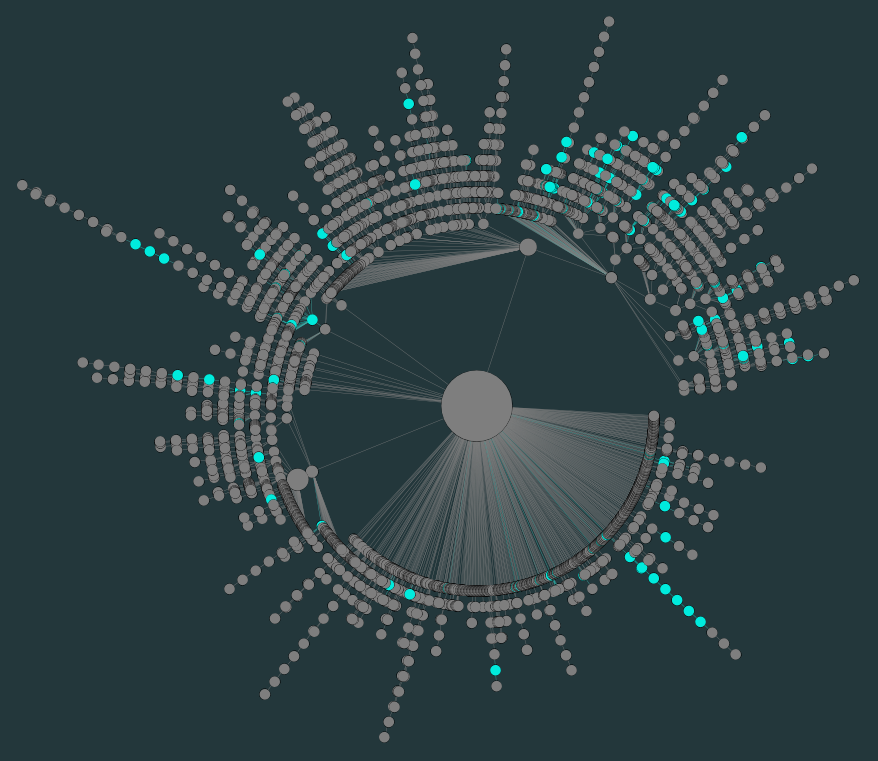
\includegraphics[width=\linewidth]{graph_dem.png}
    \caption{Thread Tree: Blue nodes are about Democrats}
    \end{figure}
  \end{column}
  \begin{column}{.5\textwidth}
    \begin{figure}[htp]
    \centering
    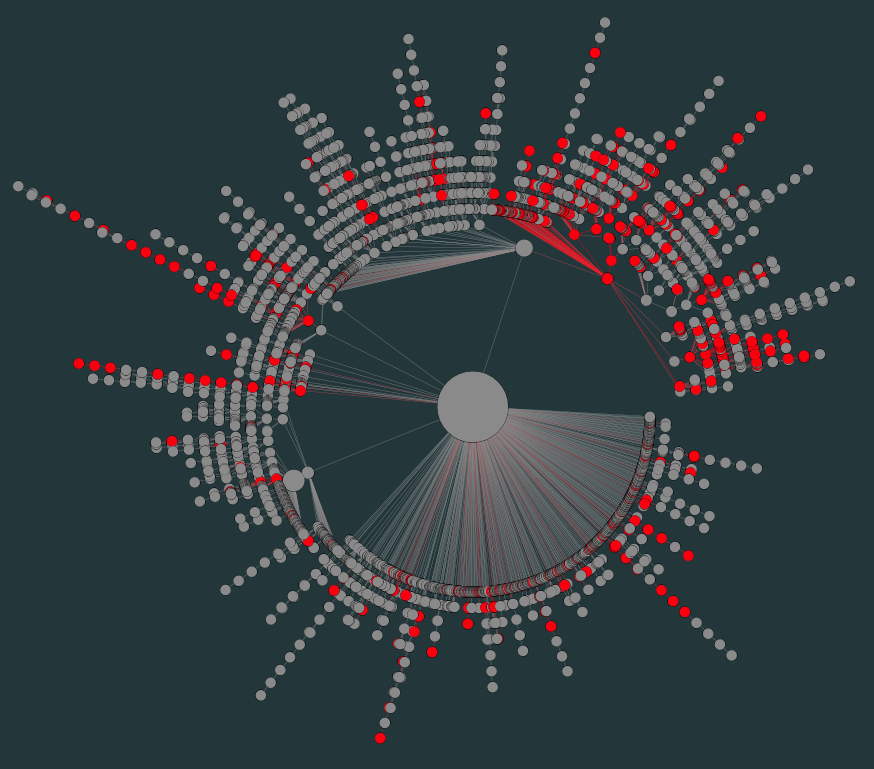
\includegraphics[width=\linewidth]{graph_rep.png}
    \caption{Thread Tree: Red nodes are about Republicans}
    \end{figure}
  \end{column}
 \end{columns}
\end{frame}

\begin{frame}{Sentiment in Thread Structure}
\begin{figure}[htp]
\centering
\movie[width=.5\textwidth, loop]{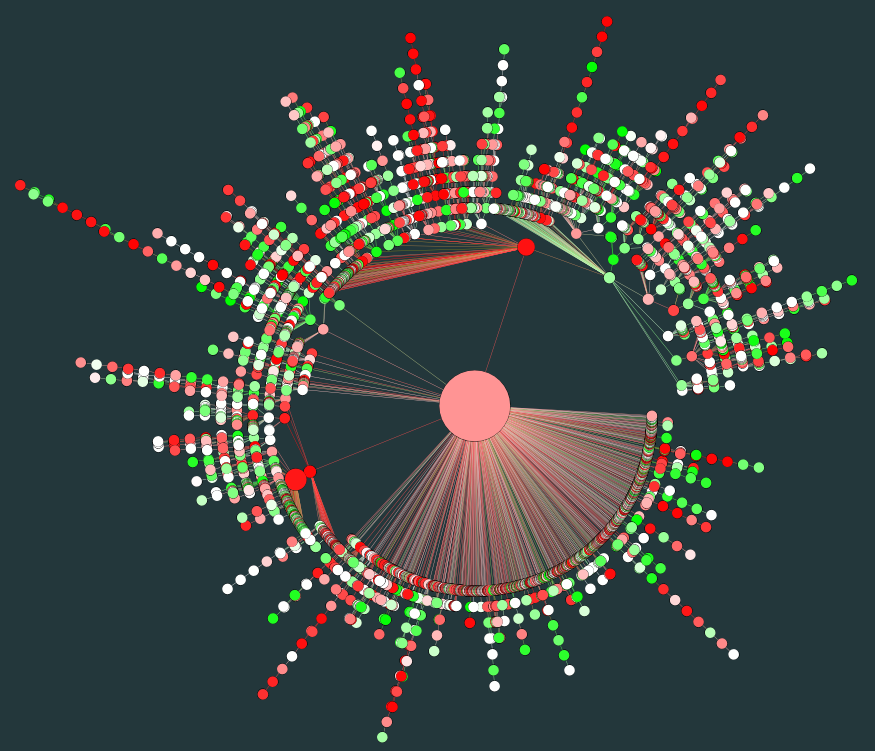
\includegraphics[width=.5\textwidth]{graph_sent.png}}{graph_evo.avi}
\caption{Thread Tree: Red nodes indicate negative sentiment, green nodes positive}
\end{figure}
\end{frame}

\section{Comment/Subreddit Analysis Over Time}

\begin{frame}
 \begin{figure}[htp]
 \centering
 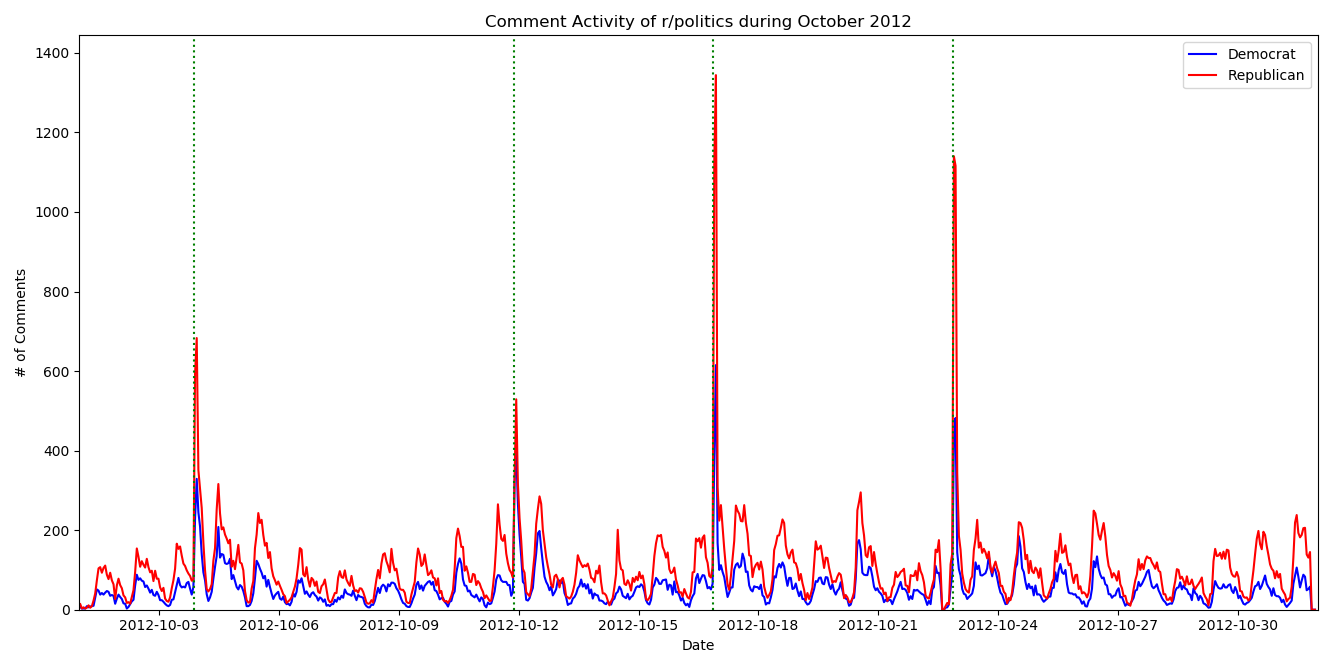
\includegraphics[width=\linewidth]{comment_activity.png}
 \caption{Number of posted comments during October 2012}
\end{figure}
\end{frame}

\begin{frame}{First Debate - 03/10/2012}
 \begin{figure}[htp]
 \centering
 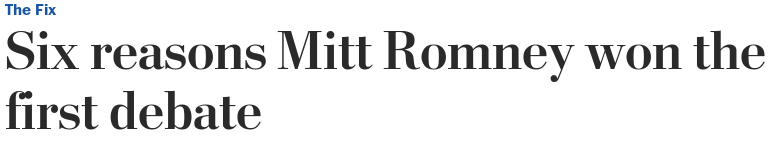
\includegraphics[width=\linewidth]{first_debate.png}
 \caption{Washington Post's article about the first presidential debate of 2012\footnotemark}
\end{figure}
\footcitetext{first_debate}
\end{frame}

\begin{frame}{Vice-President Debate - 11/10/2012}
 \begin{figure}[htp]
 \centering
 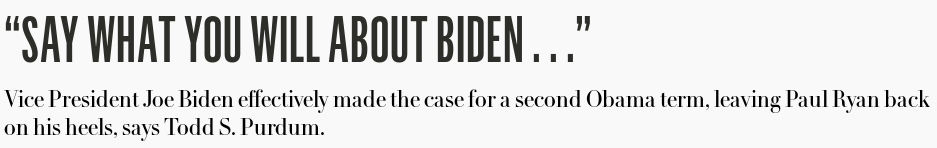
\includegraphics[width=\linewidth]{vp_debate.png}
 \caption{Vanity Fair's article about the vice-presidential debate of 2012\footnotemark}
\end{figure}
\footcitetext{vp_debate}
\end{frame}

\begin{frame}{Second Debate - 16/10/2012}
 \begin{figure}[htp]
 \centering
 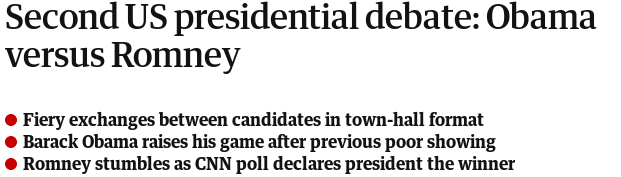
\includegraphics[width=\linewidth]{second_debate.png}
 \caption{The Guardian's article about the second presidential debate of 2012\footnotemark}
\end{figure}
\footcitetext{second_debate}
\end{frame}

\begin{frame}{Third Debate - 22/10/2012}
 \begin{figure}[htp]
 \centering
 
\includegraphics[width=\linewidth]{third_debate.png}
 \caption{Rolling Stone's article about the third and final presidential debate of 2012\footnotemark}
\end{figure}
\footcitetext{third_debate}
\end{frame}


\begin{frame}{Overall Sentiment Score}
 \(t_i^{dem}\) - Submission times of i-th comment about Democrats\\
 \(s_i^{dem}\) - Sentiment scores of i-th comment about Democrats\\
 \(u_i^{dem}\) - Upvotes for i-th comment about Democrats\\
 \pause
 To capture the general population's opinion using upvotes, consider for each hour h:\\
 \begin{equation}
  w_i^{dem} = s_i^{dem} \cdot  u_i^{dem}
 \end{equation}\pause
 \begin{equation}
  pos_{h}^{dem} = \sum_{i \in h}w_i^{dem}, \text{for } w_i^{dem}>0
 \end{equation}\pause
 \begin{equation}
  neg_{h}^{dem} = \sum_{i \in h}w_i^{dem}, \text{for } w_i^{dem}<0
 \end{equation}\pause
 \begin{equation}
  polarity_h^{dem} = 2\times \frac{\left | pos_h^{dem} \right |}{\left | pos_h^{dem} \right | + \left | neg_h^{dem} \right |}-1
 \end{equation}
\end{frame}

\begin{frame}
\only<1>{Several events can be identified due to variations in sentiment}
\only<2>{03/10 - Romney 'wins' first debate}
\only<3>{03/10 - Following days Obama's sentiment decreases}
\only<4>{15/10 - The Economist publishes statistics that encourage Obama administration}
\only<5>{16/10 - Hillary Clinton on Benghazi: 'I take responsability'}
\only<6>{16/10 - Second Presidential Debate, a more 'agressive' Obama calls out Romney}
\only<7>{21/08 - More information about the Benghazi attacks is published}
\only<8>{22/10 - Third Presidential Debate - Obama 'controlled the debate'}
 \begin{figure}[htp]
 \centering
 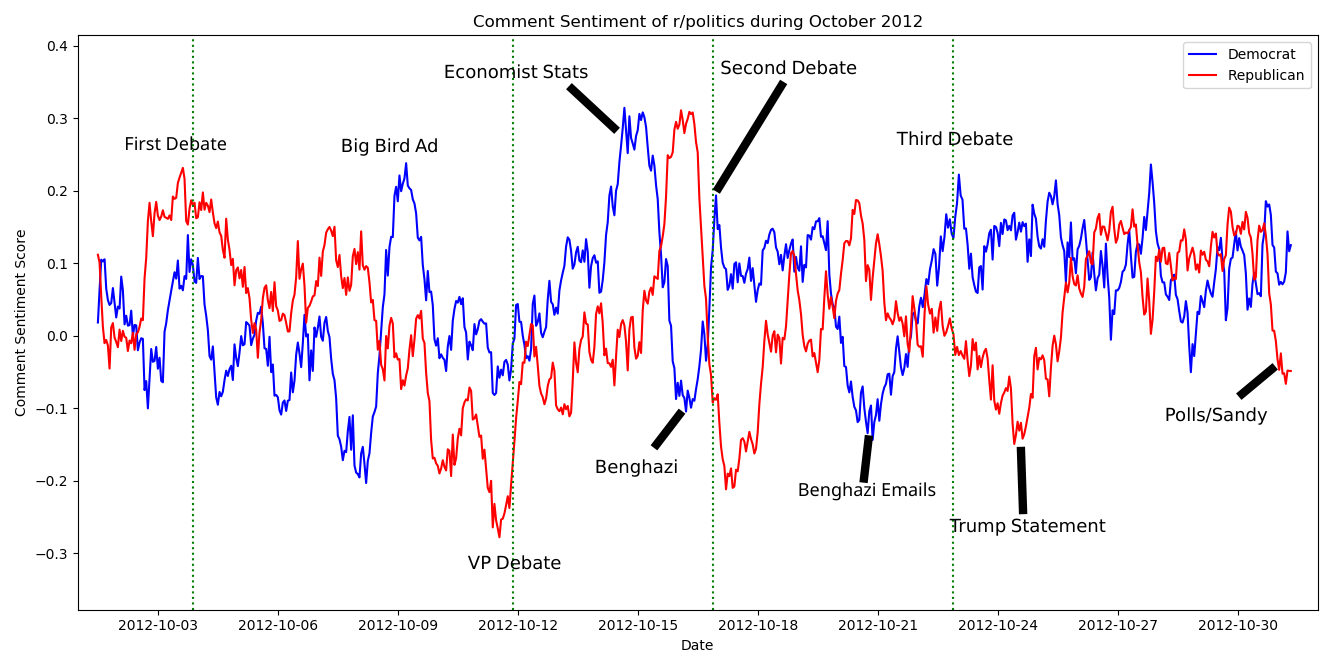
\includegraphics[width=\linewidth]{comment_sentiment_politics.png}
 \caption{Overall Sentiment of r/politics during October 2012}
\end{figure}
\end{frame}

\begin{frame}
\only<1>{Its also possible to analyse 'live' reactions to a debate}
\only<2>{The second debate, on 16/10, was the most popular and active}
\only<3>{Similar analysis as before, but considering 1-minute intervals}
\only<4>{Several debate highlights are translated as peaks or valleys}
 \begin{figure}[htp]
 \centering
 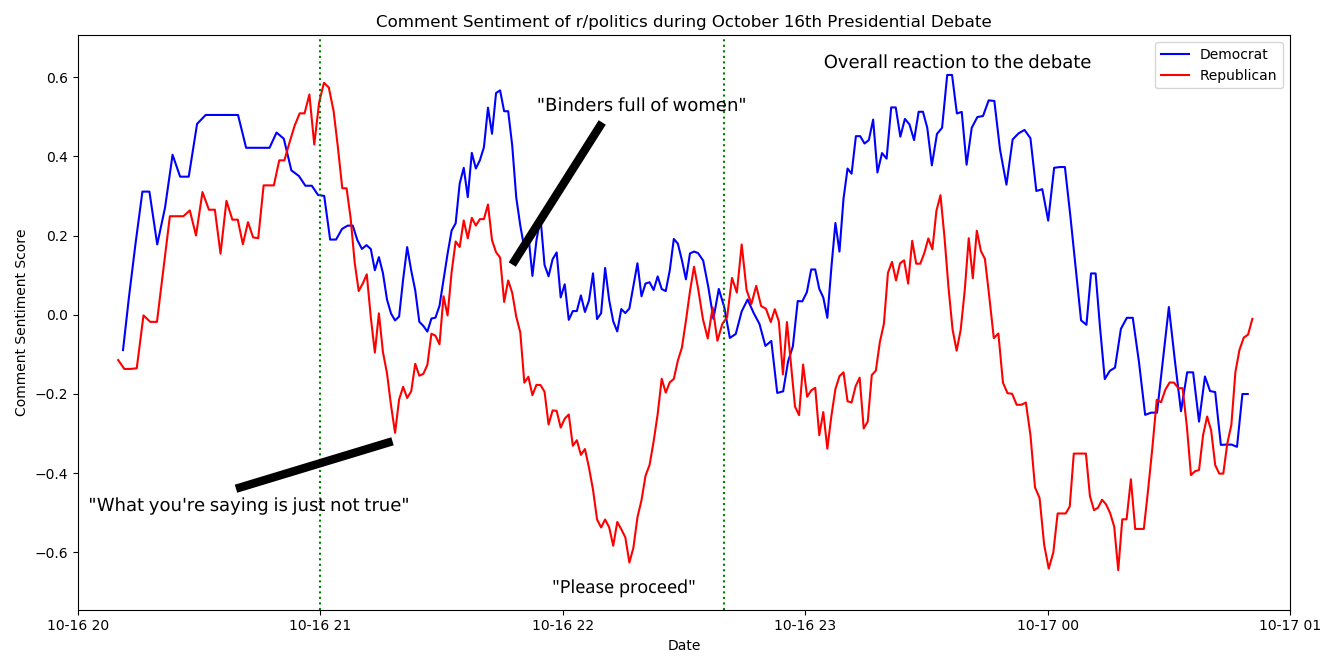
\includegraphics[width=\linewidth]{comment_sentiment_debate.png}
 \caption{Overall Sentiment of r/politics during the October 16th Debate}
\end{figure}
\end{frame}

\section{Conclusions}

\begin{frame}
 \begin{itemize}
  \item Overall Reddit Community is \alert{left-leaning}\pause
  \item Other ideologies resort to subreddits\pause
  \item Score variations tend to be symmetric \(\Rightarrow\) \alert{Confrontational} setting\pause
  \item \alert{Debates} are key events for the public opinion\pause
  \item Social News Web Sites provide an \alert{immediate insight} to current events\pause
 \end{itemize}

\end{frame}

\metroset{background=light}
\usebeamercolor[fg]{normal text}
\begin{frame}
\centering
\Huge
Thank you for your attention!
\end{frame}

\begin{frame}[allowframebreaks]
 \nocite{*}
 \printbibliography
\end{frame}


\end{document}
